%Metodología de investigación
\section{Metodología de investigación}
Con base en los niveles de maduración tecnológica del ministerio de Ciencia, Tecnología e Innovación colombiano, tomando en cuenta que se busca el desarrollo de un software que busca el aprendizaje y fortalecimiento de las habilidades blandas de los educandos de ingeniería en sistemas, ahora bien y basado en los niveles de maduración tecnológica clasificados por Minciencias, este proyecto se encuentra actualmente en el nivel TRL 3, lo que significa que está en la etapa donde se llevan a cabo pruebas de laboratorio, utilizando el ordenador como ambiente de prueba, para validar la funcionalidad de la tecnología que se está aplicando, pero que se espera que con base en el objetivo de este proyecto en el transcurso de (8) meses se alcance el nivel TRL 7.\cite{o}

\begin{figure}[ht]
  \centering
  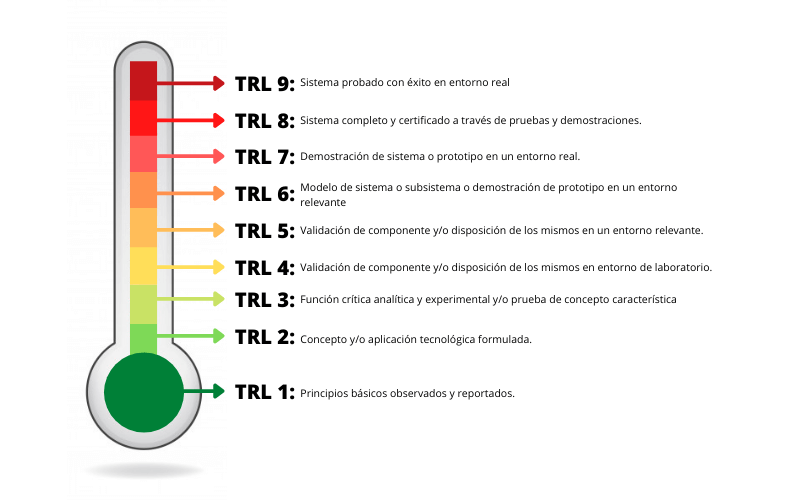
\includegraphics[width=0.8\linewidth]{Imagenes/COL.png}
  \caption{Extraida de Ayming\cite{o}}
  \label{fig:imagen2}
\end{figure}
\newpage


Considerando esto, la metodología de investigación planteada para el proyecto consistió en seguir etapas secuenciales para asegurar un proceso eficaz.
\\ \\
En primer lugar, se llevó a cabo una búsqueda bibliográfica con el fin de recopilar información pertinente acerca del desarrollo de las habilidades seleccionadas, los métodos educativos y las tecnologías de enseñanza disponibles. Esto con el objetivo de tener un conocimiento más sólido a la hora de diseñar el software. Cabe mencionar que, por consiguiente, durante esta etapa se seleccionaron las habilidades blandas a abordar.
\\ \\
Tras la finalización de la investigación, se procedió a la etapa de diseño y desarrollo del software para el aprendizaje y fortalecimiento de habilidades blandas a través de las diferentes tecnologías web y herramientas de desarrollo necesarias.
\\ \\
Después de la fase de desarrollo, se llevó a cabo la recolección de datos y evaluación utilizando diferentes medios, como encuestas y evaluaciones de desempeño. Esto permitió valorar la eficacia del software en el desarrollo de habilidades blandas. Una vez recopilada toda la información, se analizaron los datos para extraer conclusiones y generar recomendaciones de ajustes o posibles cambios futuros en la plataforma.


%Metodología de desarrollo de software
\section{Metodología de desarrollo de software}
Para el desarrollo de este proyecto se optó por una metodología ágil basada en la  necesidad de flexibilidad y eficiencia en el desarrollo del software básico para una tesis. Estos proyectos suelen enfrentar cambios en los requisitos y desafíos emergentes, por lo que requieren un enfoque adaptable que permite realizar ajustes constantes a lo largo del proceso.
\\ \\
La naturaleza volátil y cambiante de estos proyectos se encuentra en las metodologías ágiles como Scrum o Kanban. Este enfoque permite enfrentar la incertidumbre al enfocarse en principios como la simplicidad, la retroalimentación continua y la adaptación al cambio.
\\ \\
Una de las principales ventajas de Kanban radica en su enfoque visual y su capacidad para gestionar el flujo de trabajo de manera eficiente. Al utilizar columnas que representan etapas de trabajo y límites de trabajo en proceso (WIP), Kanban permite una visualización clara de las tareas en curso y ayuda a identificar cuellos de botella o áreas para mejorar la eficiencia. Esto facilita una rápida adaptación a los cambios en la demanda o prioridades del proyecto.
\\ \\
Mientras tanto Scrum se enfoca en la división del trabajo en iteraciones manejables, conocidas como sprints, facilita un proceso iterativo e incremental para la entrega del producto final, priorizando las necesidades esenciales y ajustando el enfoque conforme avanza el proyecto.
\\ \\
Para este proyecto, se ha optado por usar Scrumban, el cual fusiona las cualidades más destacadas de Scrum y Kanban. Combina la estructura orientada de Scrum con la flexibilidad y capacidad de adaptación de Kanban. 
\\ \\
“Scrumban se desarrolló inicialmente para ayudar a los equipos en su transición de Scrum a Kanban o viceversa. Si los equipos tienen más experiencia con una de las estrategias que con la otra, esta técnica les servirá para cambiar gradualmente de una metodología a otra. 
\\ \\
Si bien el motivo inicial por el que nació Scrumban fue para ayudar a que los equipos migren de un método al otro, en algunos casos, se descubrió que esta combinación de ambas estrategias resultaba beneficiosa.”\cite{p}
\\ \\
Además, al manejar cambios en los requisitos de manera efectiva, Scrumban permite realizar ajustes rápidos y eficaces incluso en etapas avanzadas del proyecto, lo que posibilita la constante mejora y optimización del software, minimizando así problemas futuros.

%Metodología de gestión de actividades
\section{Metodología de gestión de actividades}
Para la administración de las diferentes actividades y una visualización clara del flujo de trabajo se optó por el uso de tablero kanban puesto que esta herramienta, al igual que la metodología de desarrollo Scrumban , ofrece una mayor flexibilidad para adaptarse a las cambiantes necesidades del proyecto.

\section{Metodología de gamificacion}
Para una correcta aplicación de la gamificación se utilizaron una serie de técnicas mecánicas y dinámicas extraídas de dinámicas de juegos, las cuales incluyeron desafíos, misiones, logros y competiciones. Los desafíos representaron competiciones entre usuarios con el objetivo de obtener premios. Por otro lado, las misiones o retos implicaron resolver o superar objetivos planteados, ya sea individualmente o en equipo, promoviendo el logro personal y la satisfacción al alcanzarlos.
\\ \\
Los logros dentro de la gamificación educativa fueron resultados que contribuyeron a la superación individual y proporcionaron una sensación de satisfacción personal al cumplir metas específicas. La competición en este contexto implicó la búsqueda constante de mejorar y superar desafíos.
\\ \\
Es importante destacar que la esencia de la gamificación educativa no residió en la creación de juegos per se, sino en la implementación inteligente de sistemas como la puntuación, las recompensas y los objetivos que comúnmente se encuentran en los juegos. Estos elementos se utilizaron estratégicamente para fomentar la participación, el compromiso y el aprendizaje en entornos educativos.
